\documentclass[11pt]{report}

\usepackage[utf8]{inputenc} % Required for inputting international characters
\usepackage[T1]{fontenc} % Output font encoding for international characters
\usepackage[a4paper, total={7in, 10in}]{geometry}
\usepackage{mathpazo} % Palatino font
\usepackage{graphicx}
\usepackage{sectsty}
\usepackage{lipsum} 
\usepackage{pgfgantt}
\usepackage{afterpage}
\usepackage{wrapfig}
% \usepackage{indentfirst}
\usepackage{float}
\usepackage{framed}
\usepackage[pagestyles]{titlesec}
\renewcommand\bibname{References}
% \titleformat{\chapter}{\bfseries\centering}{}{0pt}{\Huge}
\titleformat{\chapter}[display]
  {\normalfont\huge\bfseries}
  {}
  {0pt}
  {\filcenter\Huge\scshape}
\titlespacing*{\chapter}{0pt}{40pt}{40pt}
\titleformat*{\section}{\Large\bfseries}
\titleformat*{\subsection}{\large\bfseries}

\renewcommand*\footnoterule{}
% \newpagestyle{mystyle}
% {\sethead[\thepage][][\chaptertitle]{}{}{\thepage}}
% \pagestyle{mystyle}
\pagestyle{plain}
\setlength{\FrameSep}{10pt}
\setlength{\FrameRule}{1pt}
\newcommand{\HRule}{\rule{\linewidth}{1pt}\bigskip\par}
% \allsectionsfont{\centering}

\begin{document}
\begin{center}
\textbf{\LARGE\textsc{Department of Computer Science and Engineering}}\bigskip\\
\textbf{\Large{VIII Semester Project}}\bigskip\\
\textbf{\huge\textsc{Monthly Progress Report - I}}\bigskip\\
\end{center}
\begin{framed}
\noindent \large{Batch No. }\hspace{64pt}\textbf{\large{35}}\medskip\\
\large{Title of the project: }\hspace{17pt}\textbf{\large\textsc{Image Regeneration using Generative Models}}\medskip\\
\noindent\begin{tabular}{@{}l@{\hspace{31pt}}l r }
\large{Team members: }  & {\large \textbf{Abhijith C.}}       & \large \textbf{1MV14CS004} \\
                        & {\large \textbf{Raghava G. Dhanya}} & \large \textbf{1MV14CS077} \\
                        & {\large \textbf{Shashank S.}}       & \large \textbf{1MV14CS131}
\end{tabular}\\[15pt]  
\noindent \large{Name of the Guide: }\hspace{12pt}\textbf{\large{Sushila Shidnal}}\medskip\\
\noindent \large{Duration: }\hspace{65pt}\textbf{\large{From February Week 3 to March Week 1}}\medskip\\
\HRule
\noindent \textbf{\Large{Details Of Work Carried Out:}}\bigskip\\
\indent Under Basic GAN, we implemented the DCGAN architecture from Alec Radford \textit{et al}\footnotemark[1]. We were able to reproduce the results on the MNIST dataset, which is a handwritten digit database with a high degree of visual accuracy. The training with CelebA dataset, a dataset of celebrity faces which has 200k examples each with 28x28 pixels, took around 30 hours to complete 1600 epochs on a modest home computer system.\par
\begin{wrapfigure}{l}{0.3\textwidth}
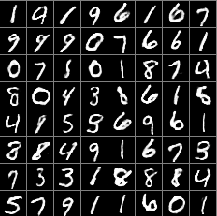
\includegraphics[width=.3\textwidth]{MNIST.png}
\caption{GAN output after 40000 epochs on MNIST}
\label{fig:MNIST}
\end{wrapfigure} 
Seeing as the training would take an enormous amount of time on standard computing systems we searched for other options. After considering AWS and Google Colaboratory, we decided on Colaboratory for its ease of use. It allows us to implement code in the form of Jupyter notebooks stored on the Google drive. Colaboratory has Nvidia Tesla GPU back-end support and 13 GB of RAM which helps improve the training speeds. For comparison it took 70 minutes to train the same DCGAN on MNIST dataset which has 60000 examples each with 28x28 pixels for 60000 epochs. This had a speedup of about 8x, even if the number of epochs are ignored. We can see the results in figure \ref{fig:MNIST}.\par
The next step in the process was to implement a vanilla CapsNet. This would act as the base code which we will augment to finally shape it into a GAN. We implemented CapsNet architecture similar to that of in Geoffrey Hinton \textit{et al.}\footnotemark[2]. We were able to reproduce the results but with longer training times. This code will be used to build a binary classifier to make it into the discriminator component of the GAN.
\end{framed}
\footnotetext[1]{Alec Radford, Luke Metz, and Soumith Chintala. Unsupervised representation learning with deep
convolutional generative adversarial networks. CoRR, abs/1511.06434, 2015.}
\footnotetext[2]{Sara Sabour, Nicholas Frosst, and Geoffrey E Hinton. Dynamic routing between capsules. In I. Guyon, U. V. Luxburg, S. Bengio, H. Wallach, R. Fergus, S. Vishwanathan, and R. Garnett, editors, Advances in Neural Information Processing Systems 30, pages 3856–3866. Curran Associates, Inc., 2017.}
\afterpage{
\begin{framed}
\noindent \textbf{\Large{Time-line:}}\\[10pt]

\includegraphics[width=1.1\textwidth]{timeline.png}\\[10pt] 
\noindent\HRule
\vspace{50px}
\centering
\textbf{Head of the Department}
\vspace{50px}
\flushleft\textbf{Project Guide}\hfill\textbf{Project Coordinator}
\end{framed}
}
\end{document}